\documentclass[11pt,varwidth=\maxdimen]{standalone}
%\documentclass{article}
\usepackage[english]{babel}	
\usepackage[utf8]{inputenc}	% Allows for writing special charachters in the tex-file 

\usepackage{amsfonts,amsmath,amssymb,bm,mathrsfs,mathtools,dsfont} 	% Standard mathematics 

% Fonts
% \DeclareMathAlphabet{\mathsfit}{OT1}{lmss}{m}{sl}
% \DeclareMathAlphabet{\mathsfbf}{OT1}{lmss}{bx}{n}
% \DeclareMathAlphabet{\mathsfbfit}{OT1}{lmss}{bx}{sl}
 
% \DeclareMathVersion{sectionmath}
% \SetSymbolFont{operators}{sectionmath}{OT1}{cmbr}{m}{n}
% \SetSymbolFont{letters}{sectionmath}{OML}{cmbrm}{b}{it}
% \SetSymbolFont{symbols}{sectionmath}{OMS}{cmbrs}{m}{n}
% \DeclareMathVersion{normalmath}
% \SetSymbolFont{operators}{normalmath}{OT1}{cmbr}{m}{n}
% \SetSymbolFont{letters}{normalmath}{OML}{cmbrm}{m}{it}
% \SetSymbolFont{symbols}{normalmath}{OMS}{cmbrs}{m}{n}

% \mathversion{normalmath}
% \renewcommand{\familydefault}{\sfdefault} %Use sans serif 


\usepackage{xcolor}
\definecolor{rmp}{RGB}{41, 43, 133}
\definecolor{myblue}{rgb}{0.24, 0.36, 0.44}
\definecolor{mygreen}{rgb}{0.367, 0.473, 0.0}


\usepackage{tikz}
\usetikzlibrary{positioning,shapes,calc,arrows.meta}
\newcommand{\coord}[4]{({(#1)+(#3)*cos(#4)},{(#2)+(#3)*sin(#4)})}


\newcommand{\sscript}[1]{{\scriptscriptstyle \mathrm{#1}}}
\newcommand{\EFT}{\sscript{EFT}}


% % % % % % Commands % % % % % % %

\begin{document}
	% Normal page width =15.4
	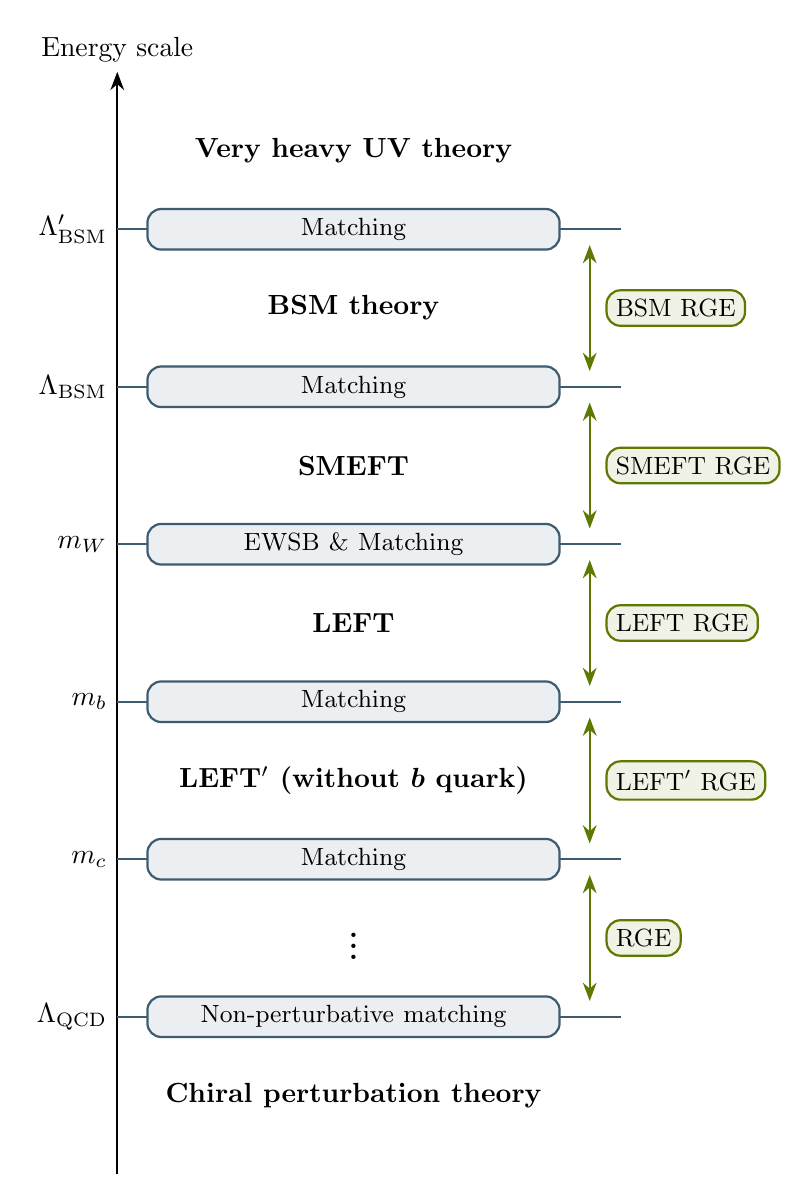
\begin{tikzpicture} [
			scale = 1,
			>={Stealth[]},
			frame/.style={draw, 
					rectangle, 
					text centered, 
					minimum size=1ex, 
					rounded corners= 5pt,
					draw= myblue,
					fill= myblue!10!white},
            frame2/.style={draw, 
					rectangle, 
                    right,
					text centered, 
					minimum size=1ex, 
					rounded corners= 5pt,
					draw= mygreen,
					fill= mygreen!10!white},
			output/.style={frame, 
%					draw= darkred, 
%					fill= darkred!20!white,
				},
			to/.style={->, line width= 1.5pt}
		] \pgfsetlinewidth{.8pt} %Set default linewidth to be thick

        % energy axis
        \node[above] at (0,14) {Energy scale}; 
        \draw[->] (0,0) -- (0,14);
        % \draw[-, myblue] (0,14) -- (6.4,14);
        \draw[-, myblue] (0,12) -- (6.4,12);
        \draw[-, myblue] (0,10) -- (6.4,10);
        \draw[-, myblue] (0,8) -- (6.4,8);
        \draw[-, myblue] (0,6) -- (6.4,6);
        \draw[-, myblue] (0,4) -- (6.4,4);
        \draw[-, myblue] (0,2) -- (6.4,2);

        % nodes on axis
        % \node[left] at (0,14) {$\Lambda_\mathrm{BSM}^\prime$};
        \node[left] at (0,12) {$\Lambda_\mathrm{BSM}^\prime$};
        \node[left] at (0,10) {$\Lambda_\mathrm{BSM}$};
        \node[left] at (0,8) {$m_{W}$};
        \node[left] at (0,6) {$m_b$};
        \node[left] at (0,4) {$m_c$};
        \node[left] at (0,2) {$\Lambda_\mathrm{QCD}$};

        % Theories
        % \node[] at (3,15) {\bf Very heavy UV theory};
        \node[] at (3,13) {\bf Very heavy UV theory};
        \node[] at (3,11) {\bf BSM theory};
        \node[] at (3,9) {\bf SMEFT};
        \node[] at (3,7) {\bf LEFT};
        \node[] at (3,5) {\bf LEFT$^\prime$ (without $\boldsymbol{b}$ quark)};
        \node[] at (3,3) {\bf \vdots};
        \node[] at (3,1) {\bf Chiral perturbation theory};
        
        % Matching
        % \node[frame, text width= 5cm] at (3,14) {\small Matching};
        \node[frame, text width= 5cm] at (3,12) {\small Matching};
        \node[frame, text width= 5cm] at (3,10) {\small Matching};
        \node[frame, text width= 5cm] at (3,8) {\small EWSB \& Matching};
        \node[frame, text width= 5cm] at (3,6) {\small Matching};
        \node[frame, text width= 5cm] at (3,4) {\small Matching};
        \node[frame, text width= 5cm] at (3,2) {\small Non-perturbative matching};

        % Running
        % \draw[<->] (6,15.8) -- (6,14.2);
        % \draw[<->, mygreen] (6,13.8) -- (6,12.2);
        \draw[<->, mygreen] (6,11.8) -- (6,10.2);
        \draw[<->, mygreen] (6,9.8) -- (6,8.2);
        \draw[<->, mygreen] (6,7.8) -- (6,6.2);
        \draw[<->, mygreen] (6,5.8) -- (6,4.2);
        \draw[<->, mygreen] (6,3.8) -- (6,2.2);
        % labels
        % \node[frame2] at (6.2,15) {\small RGE};
        % \node[frame2] at (6.2,13) {\small BSM RGE};
        \node[frame2] at (6.2,11) {\small BSM RGE};
        \node[frame2] at (6.2,9) {\small SMEFT RGE};
        \node[frame2] at (6.2,7) {\small LEFT RGE};
        \node[frame2] at (6.2,5) {\small LEFT$^\prime$ RGE};
        \node[frame2] at (6.2,3) {\small RGE};
        
	\end{tikzpicture}
	
	
\end{document}
